% Created 2020-09-23 Wed 11:24
% Intended LaTeX compiler: lualatex
\documentclass[11pt]{article}
\usepackage{graphicx}
\usepackage{grffile}
\usepackage{longtable}
\usepackage{wrapfig}
\usepackage{rotating}
\usepackage[normalem]{ulem}
\usepackage{amsmath}
\usepackage{textcomp}
\usepackage{amssymb}
\usepackage{capt-of}
\usepackage{hyperref}
\usepackage{tabularx}
\usepackage{etoolbox}
\makeatletter
\def\dontdofcolorbox{\renewcommand\fcolorbox[4][]{##4}}
\AtBeginEnvironment{minted}{\dontdofcolorbox}
\makeatother
\usepackage[newfloat]{minted}
\usepackage{amsthm}
\theoremstyle{definition}
\newtheorem{definition}{Definition}[section]
\usepackage{unicode-math}
\usepackage{unicode}
\author{Mark Armstrong}
\date{Fall 2020}
\title{Formal languages\\\medskip
\large Principles of Programming Languages}
\hypersetup{
   pdfauthor={Mark Armstrong},
   pdftitle={Formal languages},
   pdfkeywords={},
   pdfsubject={Definition and tools for building formal languages. Introduction to semantics.},
   pdfcreator={Emacs 27.0.90 (Org mode 9.3.8)},
   pdflang={English},
   colorlinks,
   linkcolor=blue,
   citecolor=blue,
   urlcolor=blue
   }
\begin{document}

\maketitle

\section{Preamble}
\label{sec:orgb531786}
This section introduces the mathematical tools
we will use in the discussion of programming languages
as a \emph{formal} language.

Several small formal languages (not full programming languages)
are used as examples of the use of these tools.

\subsection{Table of contents}
\label{sec:org9fed79f}
\begin{scriptsize}
\begin{itemize}
\item \hyperref[sec:orgb531786]{Preamble}
\begin{itemize}
\item \hyperref[sec:org9fed79f]{Table of contents}
\item \hyperref[sec:orge39b6fa]{Notable references}
\item \hyperref[sec:orgbf1b67c]{Version history}
\begin{itemize}
\item \hyperref[sec:orge322146]{September 23rd}
\item \hyperref[sec:orgc7aa726]{September 21st}
\item \hyperref[sec:org4c813c1]{September 16th}
\item \hyperref[sec:org96611cc]{Beginning of course}
\end{itemize}
\end{itemize}
\item \hyperref[sec:org1abba4f]{Formal languages}
\begin{itemize}
\item \hyperref[sec:orgb78d534]{The usefulness of formal languages}
\item \hyperref[sec:org59c986c]{Strings}
\end{itemize}
\item \hyperref[sec:orgacaeba2]{Describing the \emph{syntax} of formal languages}
\begin{itemize}
\item \hyperref[sec:org459a083]{Regular expressions as in formal language theory}
\item \hyperref[sec:orgc996e04]{The language for a regular expression}
\item \hyperref[sec:orga0426ee]{Additional operators for more expressive regular expressions}
\item \hyperref[sec:org6d3548c]{Regular expression examples}
\item \hyperref[sec:org775a78d]{Grammars as in formal language theory}
\item \hyperref[sec:org8145865]{Notations for grammar productions in formal language theory}
\item \hyperref[sec:org5527a2b]{Conventions for grammars}
\item \hyperref[sec:org40e6ba4]{A simple example grammar}
\item \hyperref[sec:org7e41844]{Exercise – reading grammars}
\item \hyperref[sec:org4f12455]{Grammars generate or recognise strings}
\item \hyperref[sec:orga475d8c]{Parse trees}
\item \hyperref[sec:orgb22edea]{Example parse tree}
\item \hyperref[sec:org7b65470]{Another example parse tree}
\item \hyperref[sec:orgfb44648]{Exercise: creating parse trees}
\item \hyperref[sec:org7201aab]{Backus-Naur form (BNF)}
\item \hyperref[sec:orgcdc3693]{BNF details}
\item \hyperref[sec:orgee8aa97]{Aside: ALGOL}
\item \hyperref[sec:org41b6b47]{Extended Backus-Naur form (EBNF)}
\item \hyperref[sec:org326949e]{EBNF details}
\item \hyperref[sec:orgba7cfc1]{Exercise – translating to EBNF}
\item \hyperref[sec:orge66946e]{EBNF's syntactic sugar}
\item \hyperref[sec:org9cf9f20]{Exercise – a small language C-like language}
\item \hyperref[sec:org01a9da9]{Example – EBNF for C++}
\end{itemize}
\item \hyperref[sec:org68cc17f]{Parsing and executable code}
\begin{itemize}
\item \hyperref[sec:orgc07fd9a]{Atomic syntactic units}
\item \hyperref[sec:org0ea7aa0]{Lexemes and tokens}
\item \hyperref[sec:org6f52ff9]{Parsing}
\item \hyperref[sec:org9757a9b]{The zeroth step – preprocessing}
\item \hyperref[sec:org5dd76c0]{The first step – lexical analysis}
\item \hyperref[sec:org9e52d96]{The second step – parsing (syntactic analysis)}
\item \hyperref[sec:orgd94f1ec]{The third step – (static) semantic analysis}
\item \hyperref[sec:orge1d5e37]{The fourth step – intermediate code generation}
\item \hyperref[sec:orgac6abb0]{Visualising the entire parsing process}
\end{itemize}
\item \hyperref[sec:orgf4bc1ae]{Compilation, interpretation, and hybrid appraoches}
\begin{itemize}
\item \hyperref[sec:orgf94dfeb]{Compilation}
\item \hyperref[sec:orga4e2231]{Interpreters}
\item \hyperref[sec:orgfb8a43b]{Hybrid methods}
\end{itemize}
\item \hyperref[sec:org5846edf]{Ambiguity}
\begin{itemize}
\item \hyperref[sec:orgf5fa90c]{An example of ambiguity}
\item \hyperref[sec:org809ed05]{Removing ambiguity}
\item \hyperref[sec:orgfacd5ca]{Parentheses make structure clear}
\item \hyperref[sec:orgd04cbac]{Enforcing precedence with a grammar}
\item \hyperref[sec:org1bf2b64]{Enforcing associativity with a grammar}
\item \hyperref[sec:org6ad7544]{“Associative” operations}
\item \hyperref[sec:orgf9a2272]{Addition is not associative… in some cases}
\end{itemize}
\item \hyperref[sec:org82e4bfd]{Abstract and concrete syntax; setting ambiguity aside}
\begin{itemize}
\item \hyperref[sec:orgf3f4748]{Abstract syntax trees are parse trees.}
\item \hyperref[sec:orga8a2924]{We are interested in abstract syntax}
\end{itemize}
\item \hyperref[sec:org858dcd4]{The \emph{semantics} of formal languages}
\begin{itemize}
\item \hyperref[sec:org1b5b75d]{Semantic domains}
\item \hyperref[sec:orgf932e15]{Example – semantics of a language of natural numbers}
\item \hyperref[sec:orgd3c8abf]{Example – semantics of propositional logic}
\item \hyperref[sec:org61bdf84]{Example – small-step semantics of propositional logic}
\end{itemize}
\end{itemize}
\end{scriptsize}

\subsection{Notable references}
\label{sec:orge39b6fa}
\begin{itemize}
\item Benjamin Pierce,
“\href{https://ebookcentral.proquest.com/lib/mcmu/detail.action?docID=3338823}{Types and Programming Languages}”
\begin{itemize}
\item Chapter 3, Untyped Arithmetic Expressions
\begin{itemize}
\item Grammars. Alternative syntactic descriptions. Semantics.
\end{itemize}
\item Chapter 5, The Untyped Lambda-Calculus
\begin{itemize}
\item Abstract syntax.
\end{itemize}
\end{itemize}

\item Peter Van Roy and Seif Haridi,
“\href{http://citeseerx.ist.psu.edu/viewdoc/download?doi=10.1.1.102.7366\&rep=rep1\&type=pdf}{Concepts, Techniques, and Models of Computer Programming}”
\begin{itemize}
\item Section 2.1, Defining practical programming languages
\begin{itemize}
\item Grammars. Alternative semantic approach (the kernel approach.)
\end{itemize}
\end{itemize}

\item Maribel Fernández,
“\href{https://discovery.mcmaster.ca/iii/encore/record/C\_\_Rb2200622?lang=eng}{Programming Languages and Operational Semantics: A Concise Overview}” 
\begin{itemize}
\item Section 1.3, Components of a Programming Language
\end{itemize}

\item Robert W. Sebesta, “Concepts of Programming Languages” (10th edition)
\begin{itemize}
\item Chapter 3, Describing Syntax and Semantics
\item Chapter 4, Lexical and Syntax Analysis
\end{itemize}
\end{itemize}

\subsection{Version history}
\label{sec:orgbf1b67c}
\subsubsection{September 23rd}
\label{sec:orge322146}

Notes completed.

\subsubsection{September 21st}
\label{sec:orgc7aa726}

More complete version posting. Nearly complete up to
Ambiguity.

\subsubsection{September 16th}
\label{sec:org4c813c1}
More complete version posted. Nearly complete up to Parsing.

After lecture, several typos fixed.
First parse tree example also fixed
(the nodes were in the wrong order.)

\subsubsection{Beginning of course}
\label{sec:org96611cc}
Very incomplete version of the notes in place.

\section{Formal languages}
\label{sec:org1abba4f}
Recall, from formal language theory:

A language over an \emph{alphabet} (set of symbols) \(Σ\)
is a subset of \(Σ^{*}\).
The elements of a language are called \emph{sentences}
(or \emph{strings} or sometimes \emph{words}).

A \emph{formal} language is one for which we have a mathematical tool
for either
\begin{itemize}
\item \emph{generating} (or \emph{deriving}) all sentences of the language,
or equivalently,
\item \emph{recognising} (or \emph{accepting}) only sentences of the language.
\end{itemize}

Examples of such mathematical tools include
\begin{itemize}
\item regular expressions,
\item automata, and
\item grammars.
\end{itemize}

\subsection{The usefulness of formal languages}
\label{sec:orgb78d534}
Formal languages, unlike \emph{natural} languages, are well-suited
for comprehension by computers.
\begin{itemize}
\item Machines require unambiguous steps to follow.
\item Hence, all programming languages are formal languages.
\end{itemize}

In particular, in most cases:
\begin{itemize}
\item The sets of keywords, names, etc., form several \emph{regular languages},
and so can be recognised by regular expressions.
\item The set of valid (in terms of form) programs forms
a \emph{context-free} language, and so can be recognised by
a (context-free) grammar.
\end{itemize}

\subsection{Strings}
\label{sec:org59c986c}
Recall that given a set \(Σ\), the set of strings over \(Σ\),
written \(Σ^{*}\), is the set of all finite sequences
of elements of \(Σ\).

In particular, the sequence of length zero we denote by \(ε\).
Note that some other sources use \(λ\) for this purpose.

For example, for \(Σ = \{a, b, c\}\),
\begin{center}
\(Σ^{*} = \{ε, a, b, c, aa, ab, ac, ba, bb, bc, ca, cb, cc, aaa, …\}\).
\end{center}

Given an element \(e ∈ Σ\), we write
\begin{itemize}
\item \(e^{n}\) for the string consisting of \(n\) occurrences of \(e\), and
\item \(e^{*}\) for the set \(\{ n ∈ ℕ ∣ e^{n} \}\).
\end{itemize}

\section{Describing the \emph{syntax} of formal languages}
\label{sec:orgacaeba2}
In this section, we will
\begin{itemize}
\item briefly review regular expressions and grammars as
they are presented in formal language theory, and then
\item introduce more practical syntax for each
which is used in practice.
\end{itemize}

In both cases, the additional syntax only adds to
the \emph{practical expressiveness} of the tool.
\begin{itemize}
\item It does not change the tool's \emph{theoretical expressiveness}.
\begin{itemize}
\item The same set of languages can be described,
but many languages can be described “more easily”.
\end{itemize}
\item We will present brief arguments to this effect
by showing how to translate from the new syntax
to the restricted syntax.
\end{itemize}

\subsection{Regular expressions as in formal language theory}
\label{sec:org459a083}
Given a finite alphabet \(Σ\),
the set of regular expressions (over \(Σ\)),
denoted \(RE(Σ)\), is given
by the following rules.
\begin{enumerate}
\item \(∅\), \(ε\) and \(a\) (for each \(a ∈ Σ\)) are regular expressions.
\item \((α | β)\), \((αβ)\) and \((α^{*})\) are regular expressions
\begin{itemize}
\item for any regular expressions α and β.
\end{itemize}
\end{enumerate}

Respectively, the three operations in (2) are called
\begin{itemize}
\item “or”,
\item “append”, and
\item “star” or “repeat”.
\end{itemize}

\subsection{The language for a regular expression}
\label{sec:orgc996e04}
The language generated/recognised by a regular expression
is defined via a (semantic) function \(L : RE(Σ) → Σ^{*}\),
defined as follows.
\begin{itemize}
\item \(L(∅) = ∅\)
\item \(L(ε) = \{ ε \}\)
\item \(L(a) = \{ a \}\)
\item \(L(α | β) = L(α) ∪ L(β)\)
\item \(L(αβ) = \{ uv | u ∈ L(α) ∧ v ∈ L(β) \}\)
\item \(L(α^*) = (L(α))^*\)
\end{itemize}

\subsection{Additional operators for more expressive regular expressions}
\label{sec:orga0426ee}
Regular expressions come up frequently in programming,
and there is a rich set of extensions
to make them easier to construct.

We will not try to extensively list them, but some are listed below,
along with their equivalent “basic” form or,
where that is infeasible to write,
its language.
\begin{enumerate}
\item \(α^{+} \ \ \ ≈ \ \ \ αα^{*}\)
\item \(α? \ \ \ ≈ \ \ \ α | ε\)
\item \(\text{.} \ \ \ ≈ \ \ \ a | b | c | …\) where \(Σ = {a, b, c, …}\); i.e., \(L(.) = Σ\)
\item \([c_{1}…c_{n}] \ \ \ ≈ \ \ \ c_{1} | … | c_{n}\), where each \(c_{i}\) is a character.
\item \([\verb!^!c_{1}…c_{n}]\), where \(L([\verb!^!c_{1}…c_{n}]) = Σ - [c_{1}…c_{n}]\).
\item \(α\{m,n\}\), where \(L(α\{m,n\}) = ⋃_{i=m}^{n} L(α)^{i}\)
\end{enumerate}

\subsection{Regular expression examples}
\label{sec:org6d3548c}
The set of all non-empty strings over the alphabet
can be described by this regular expression.
\begin{itemize}
\item Note that if \(Σ\) includes whitespace characters,
this regular expression will allow strings made only of whitespace.
\end{itemize}
\begin{minted}[breaklines=true]{text}
.⁺
\end{minted}

The set of all non-empty strings which do not include
the letters \texttt{a}, \texttt{b} or \texttt{c} can be described by this regular expression.
\begin{minted}[breaklines=true]{text}
[^abc]⁺
\end{minted}

The set \texttt{\{na,nana,banana\}} can be described by
\begin{minted}[breaklines=true]{text}
(bana|na)(na)?
\end{minted}

\subsection{Grammars as in formal language theory}
\label{sec:org775a78d}
Formally, a context-free grammar is a 4-tuple
\begin{center}
\(⟨N, Σ, P, S⟩\)
\end{center}
where
\begin{itemize}
\item \(N\) is a finite set of \emph{non-terminal} symbols
(sometimes called variables),
\item \(Σ\) is the underlying alphabet,
also called the \emph{terminals} of the grammar,
\item \(N\) and \(Σ\) must be distinct,
\item \(P\) is a set of \emph{productions} i.e.,
a binary relation between \(N\) and \((N ∪ Σ)^{*}\),
\begin{itemize}
\item In other words, a multi-valued function from
nonterminals to strings of non-terminals and terminals,
\end{itemize}
\item \(S\) is a distinguished element of \(N\), called the \emph{starting nonterminal}.
\end{itemize}

\subsection{Notations for grammar productions in formal language theory}
\label{sec:org8145865}
Given
\begin{center}
\((A, α) ∈ P\),
\end{center}
we write
\begin{center}
\(A ⟶ α\)
\end{center}
and read it as
\begin{center}
“\(A\) produces \(α\)” or “\(A\) expands to \(α\)”.
\end{center}

Given a number of
productions
\begin{center}
\((A, α₁) ∈ P\), \((A, α₂) ∈ P\), …, \((A, αₘ) ∈ P\),
\end{center}
we write
\begin{center}
\(A ⟶ α₁ | α₂ | … | αₘ\)
\end{center}
as a shorthand.

\subsection{Conventions for grammars}
\label{sec:org5527a2b}
Writing the 4-tuple each time we produce a grammar is tedious.

For this reason, we adopt the following conventions
in order to allow us to omit the 4-tuple.
\begin{enumerate}
\item We write \emph{only} the list of productions.
\item The set \(N\) is taken to be the set of all symbols
appearing to the left of a list of productions.
\begin{itemize}
\item Note that this requires each nonterminal have
at least one production.
\end{itemize}
\item The set \(Σ\) is usually understood by the context
in which we are defining the grammer.
\begin{itemize}
\item For our purposes, it will usually be the set of
all ASCII symbols.
\end{itemize}
\item The starting nonterminal \(S\) is understood to be either
\begin{enumerate}
\item the nonterminal whose name matches that of the grammar
we are defining (it may be uncapitalised or abbreviated),
\item otherwise, the non-terminal named \(S\), or
\item otherwise, the nonterminal to the left of
the first production in the list.
\begin{itemize}
\item (We usually attempt to write grammars “top down”.)
\end{itemize}
\end{enumerate}
\end{enumerate}

\subsection{A simple example grammar}
\label{sec:org40e6ba4}
\begin{minted}[breaklines=true]{text}
A ⟶ aAa | B
B ⟶ bBb | C
C ⟶ cCc | ε
\end{minted}

This produces the language of strings of
the form
\begin{center}
\(a^{i}b^{j}c^{k}c^{k}b^{j}a^{i}\)
\end{center}

\subsection{Exercise – reading grammars}
\label{sec:org7e41844}
What languages do the following grammars produce?

\begin{minted}[breaklines=true]{text}
A ⟶ B | C
B ⟶ aaB | ε
C ⟶ aaaC | ε
\end{minted}

\begin{minted}[breaklines=true]{text}
A ⟶ aB | B | ε
B ⟶ bC | C
C ⟶ cA | A
\end{minted}

\begin{minted}[breaklines=true]{text}
A ⟶ aA | B
B ⟶ bB
\end{minted}

\textbf{What's the tricky part with the last one?}

Extra exercise: can you simplify any of them?
For instance, by having less non-terminals or less productions?
If you believe so, just be careful that
your simplification accepts the same string!

\subsection{Grammars generate or recognise strings}
\label{sec:org4f12455}
We have discussed the facts that a grammar can
\begin{itemize}
\item generate strings or
\item recognise/accept strings.
\end{itemize}

Then for a grammar \(G\) we might think of functions
\begin{itemize}
\item \(generateᴳ : ℕ → Σ^{*}\)
\begin{itemize}
\item with the intention that \(generateᴳ(n)\) generates the \(n^{th}\)
string in the grammar's language is lexicographic order
\end{itemize}
\item \(recogniseᴳ : Σ^{*} → Bool\)
\end{itemize}
That is, we have two functions, which output a \texttt{String} or
a \texttt{Bool} respectively.

But there is a useful byproduct which may be obtained during
during either process: a \emph{parse tree}.

\subsection{Parse trees}
\label{sec:orga475d8c}
A parse tree's
\begin{itemize}
\item nodes (which have children) are
labelled by a nonterminal of the grammar,
\item leaves (which do not have children) are
labelled by a terminal of the grammar, and
\item if a node is labelled by a nonterminal \texttt{A},
the children of that node must correspond to
(in order from left to right)
the terminals and nonterminals appearing in a production of \texttt{A}.
If a non-terminal would produce \texttt{ε}, it is omitted.
\end{itemize}

\subsection{Example parse tree}
\label{sec:orgb22edea}
For example, consider the grammar
\begin{minted}[breaklines=true]{text}
S ⟶ AB
A ⟶ aA | ε
B ⟶ Bb | b
\end{minted}

We have the following parse tree for the string \texttt{aab}.
\begin{itemize}
\item Note the dashed portions, which show part of how the tree
was derived from the grammar,
but which will usually be omitted by our rules for parse trees.
\end{itemize}
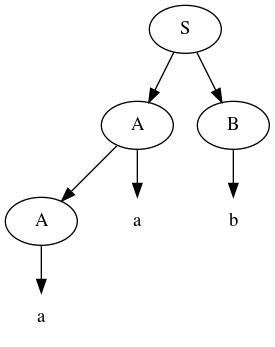
\includegraphics{media/parse-tree-example-aab.png}

\subsection{Another example parse tree}
\label{sec:org7b65470}
Similarly, working with the same grammar,
we have the following parse tree for \texttt{abb}.
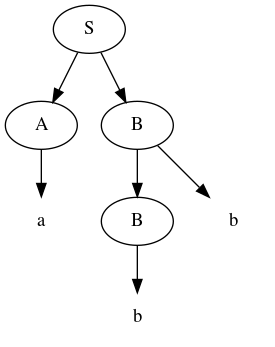
\includegraphics{media/parse-tree-example-abb.png}

\subsection{Exercise: creating parse trees}
\label{sec:orgfb44648}
Exercise: provide a parse tree for the string \texttt{aaa} using this grammar.
Is there a valid parse tree for the string \texttt{bbb}?

Exercise: if we add a production \texttt{A ⟶ a} to our example grammar,
can you provide a different parse tree
(or multiple different parse trees) for \texttt{aaa}?

\subsection{Backus-Naur form (BNF)}
\label{sec:org7201aab}
Up until now, we have used the form
\begin{verbatim}
N₁ ⟶ P₁ | P₂ | …
   ⋮
\end{verbatim}
for our production lists.

Commonly in the study of programming languages,
an alternative syntax called \emph{Backus-Naur} form (BNF)
is used.
\begin{itemize}
\item Named for two members of the ALGOL design committee,
who created the first formal definition for a programming language,
namely ALGOL.
\end{itemize}

\subsection{BNF details}
\label{sec:orgcdc3693}
In Backus-Naur form,
\begin{itemize}
\item all nonterminals names are delimited by
angle brackets, \texttt{⟨⟩},
\begin{itemize}
\item (if using ASCII characters, \texttt{<>})
\end{itemize}
\item the \texttt{⟶} is replaced by \texttt{∷=},
\item additional whitespace is permitted on the right side
of a production between terminals and nonterminals,
without changing the meaning of the production
\begin{itemize}
\item So \(⟨A⟩ ∷= a\ a\ ⟨A⟩\) is treated the same as \(⟨A⟩ ∷= aa⟨A⟩\).
\end{itemize}
\end{itemize}

\subsection{Aside: ALGOL}
\label{sec:orgee8aa97}
ALGOL (for “ALGOrithmic Language”)
was a contemporary of Fortran, Lisp, and Cobol.
\begin{itemize}
\item Together, those three are the oldest languages
still in (fairly) common use today.
\begin{itemize}
\item Granted, not the same versions.
\end{itemize}
\end{itemize}

Specifically, there were several iterations of ALGOL,
the three major ones being ALGOL 58, ALGOL 60 and ALGOL 68.

ALGOL is not in common use, but it was
the most influential on modern programming language syntax,
introducing concepts such as the block.
\begin{itemize}
\item The “C family” can trace its lineage directly to ALGOL.
\end{itemize}

\subsection{Extended Backus-Naur form (EBNF)}
\label{sec:org41b6b47}
We further extend our grammar notation to include several
several additional operators.
\begin{itemize}
\item These extensions are part of the \emph{extended} Backus-Naur form.
\item Once again, this is only an extension in the \emph{practicality} sense.
\end{itemize}

There is an \href{https://www.iso.org/standard/26153.html}{ISO standard} for EBNF.
Our syntax and inclusion of features is
not chosen to match the standard;
it is what is convenient for our use.

\subsection{EBNF details}
\label{sec:org326949e}
\begin{itemize}
\item (Square) brackets, \texttt{[]}, surrounding a string
indicate that string may or may not be included in a production.
\begin{itemize}
\item I.e., they make part of a production optional.
\item \(⟨A⟩ ∷= α₁\ [\ α₂\ ]\ α₃\ \ \ \ ≈ \ \ \ ⟨A⟩ ∷= α₁\ α₂\ α₃\ |\ α₁\ α₃\).
\end{itemize}
\item (Curly) braces, \texttt{\{\}}, surrounding a string
indicate that string may be repeated any number of times,
including zero.
\begin{itemize}
\item \(⟨A⟩ ∷= α₁\ \{\ α₂\ \}\ α₃\ \ \ \ ≈ \ \ \ ⟨A⟩ ∷= α₁\ ⟨A′⟩\ α₃\), \(⟨A′⟩ ∷= α₂\ ⟨A′⟩\ |\ ε\).
\end{itemize}
\item Parentheses, \texttt{()}, may group parts of a string.
\item The “alternative” pipe, \texttt{|}, may be used \emph{inside} of productions,
to indicate alternatives inside a set of brackets, braces
or parentheses.
\begin{itemize}
\item \(⟨A⟩ ∷= α₁\ (α₂\ |\ α₃)\ α₄ \ \ \ ≈ \ \ \ ⟨A⟩ ∷= α₁\ α₂\ α₄\ |\ α₁\ α₃\ α₄\).
\end{itemize}
\item Where necessary, terminals may be single or double quoted,
such as to indicate a whitespace character, pipe or quote.
\begin{itemize}
\item \(⟨\text{ebnfprods}⟩ ∷= ⟨\text{string}⟩\ |\ ⟨\text{string}⟩\ ⟨\text{optws}⟩\ “|”\ ⟨\text{optws}⟩\ ⟨\text{ebnfprods}⟩\)
\end{itemize}
\end{itemize}

\subsection{Exercise – translating to EBNF}
\label{sec:orgba7cfc1}
Translate this grammar from an earlier exercise to EBNF syntax.
\begin{minted}[breaklines=true]{text}
A ⟶ B | C
B ⟶ aaB | ε
C ⟶ aaaC | ε
\end{minted}
Then try to reduce the number of productions in the grammar,
while maintaining the language defined.

Can you use only one production when using EBNF?

\subsection{EBNF's syntactic sugar}
\label{sec:orge66946e}
EBNF and our extended regular expressions syntax
give us our first example of \emph{syntactic sugar};
syntax that does not add new features to a language,
only more convenient notation.
\begin{itemize}
\item As shown above, any grammar using the additional operators
can be translated into one not using them.
\begin{itemize}
\item But this likely requires more productions.
\item And certainly more characters/space on the page.
\end{itemize}
\end{itemize}

Syntactic sugar is a common feature of programming languages.
\begin{itemize}
\item Example: (imperative) languages often include various kinds of loops,
where only one (or sometimes none!) is truly necessary.
\end{itemize}

When we discuss programming languages formally,
we will usually omit constructs which are syntactic sugar.
\begin{itemize}
\item If anything, we may note how to represent them
in a “core” language which includes less constructs.
\end{itemize}

\subsection{Exercise – a small language C-like language}
\label{sec:org9cf9f20}
Consider the following context-free language.
\begin{verbatim}
⟨stmt⟩   ∷= ⟨assign⟩ | ⟨stmt⟩ "; " ⟨stmt⟩
⟨stmt⟩   ∷= "while " ⟨expr⟩ " do " ⟨stmt⟩ | ⟨ws⟩ ⟨stmt⟩ ⟨ws⟩
⟨assign⟩ ∷= ⟨var⟩ ⟨ws⟩ " := " ⟨expr⟩
⟨expr⟩   ∷= ⟨var⟩ | ⟨const⟩ | ⟨expr⟩ ⟨op⟩ ⟨expr⟩ | ⟨ws⟩ ⟨expr⟩ ⟨ws⟩
⟨var⟩    ∷= ('x' | 'y' | 'z') {⟨var⟩}
⟨const⟩  ∷= (1 | 2 | 3 | 4 | 5 | 6 | 7 | 8 | 9 | 0) {⟨const⟩}
⟨op⟩     ∷= '+' | '-' | '*' | '/' | '<' | '>' | '='
⟨ws⟩     ∷= {' '} | {'\n'}
\end{verbatim}

Provide some example programs in this language.

Can you precisely describe the language in English?

\subsection{Example – EBNF for C++}
\label{sec:org01a9da9}
A good example of the practicality EBNF for specifying
the syntax of languages is this
\href{http://www.externsoft.ch/download/cpp-iso.html}{EBNF grammar for C++}
(presented in tabular form, rather than lists of productions
as we use).

The grammar is much, much larger than anything we will write,
but it is still quite concise for describing
a real-world programming language.

\section{Parsing and executable code}
\label{sec:org68cc17f}
We will briefly summarise the parsing process,
beginning with some important terms.
\begin{itemize}
\item In this course, we are primarily interested in
the beginning of this process, up to the
construction of parse trees.
\end{itemize}

\subsection{Atomic syntactic units}
\label{sec:orgc07fd9a}
We have mentioned that both regular expressions and
context-free grammars are used in the description of
the syntax of programming languages.

However, our example programming language earlier
was described exclusively by a context-free grammar.
\begin{itemize}
\item Even the smallest syntactic units of the language,
the \emph{atomic} syntactic units, have been described by the grammars.
\begin{itemize}
\item For instance, we have used the production
\(⟨const⟩  ∷= (1 | 2 | 3 | 4 | 5 | 6 | 7 | 8 | 9 | 0) \{⟨const⟩\}\)
which describes numerical constants.
\end{itemize}
\end{itemize}

This is not done in practice.

\subsection{Lexemes and tokens}
\label{sec:org0ea7aa0}
In practice,
\begin{itemize}
\item regular expressions are instead used to describe the
atomic syntactic units of languages.
\begin{itemize}
\item For example,
\begin{itemize}
\item keywords such as \texttt{if} and \texttt{while}, constant values such as \texttt{0} or \texttt{"abc"},
or names such as \texttt{height} or \texttt{sqrt}.
\end{itemize}
\item Lexemes cannot be broken down into meaningful pieces.
\end{itemize}
\item Grammars are then used to describe the possible arrangements
of lexemes.
\begin{itemize}
\item The terminals of the grammar are then names for sets of lexemes,
called \emph{tokens}, rather than elements of \(Σ\).
\item For instance,
\begin{itemize}
\item the token \texttt{while} for the set containing only the
keyword \texttt{while},
\item or the token \texttt{int\_literal} for the set \(\{ 0, 1, -1, 2, … \}\),
\item or the token \texttt{var} for the set of valid variable names.
\end{itemize}
\end{itemize}
\end{itemize}

\subsection{Parsing}
\label{sec:org6f52ff9}
Parsing is the process of translating a program
from plaintext to executable instructions
\begin{itemize}
\item whether this is done
\begin{itemize}
\item ahead of time (compiling) or
\item when the program is to be run (interpreting),
\end{itemize}
parsing is a necessary step before execution.
\item A computer cannot run unparsed higher level language code.
\end{itemize}

\subsection{The zeroth step – preprocessing}
\label{sec:org9757a9b}
Many programming languages support some form
of \emph{preprocessing directives} which are
to be carried out before the parsing process
properly begins.
\begin{itemize}
\item Commonly, “macros”, which often are simply
textual substitutions to be carried out.
\begin{itemize}
\item But they can be used for significantly more;
in some instances, these directives
form a programming language themselves.
\end{itemize}
\end{itemize}

\subsection{The first step – lexical analysis}
\label{sec:org5dd76c0}
After preprocessing, if it is present, comes the
the conversion of the plaintext source code
into a sequence of \emph{tokens}.
\begin{itemize}
\item This process may be
called \emph{lexical analysis}, \emph{lexing} or \emph{tokenising}.
\item The program to carry this process out may be
called a \emph{lexer} or \emph{tokeniser}.
\item Lexical analysis discards whitespace, comments, and any other
text which is irrelevant to the machine.
\end{itemize}

\subsection{The second step – parsing (syntactic analysis)}
\label{sec:org9e52d96}
After converting from plaintext to a string of tokens, the next
step of parsing is to construct the parse tree.

This step is part of the parsing process,
but it is also usually called parsing.
\begin{itemize}
\item It may also be called \emph{syntactic analysis}.
\end{itemize}

More information about the program may be discarded here,
as the structure of the tree makes certain text
irrelevant (such as parentheses).

\subsection{The third step – (static) semantic analysis}
\label{sec:orgd94f1ec}
Once the parse tree is constructed,
rules about the form of programs
which cannot be (or cannot easily be)
described by a grammar are enforced
by \emph{(static) semantic analysis}.

These rules include type checking and variable scope checking,
issues we will discuss later in the course.

This process produces the \emph{symbol table}, which maps
each identifier to its relevant information,
such as
\begin{itemize}
\item where it is declared in the source and
\item its type.
\end{itemize}

\subsection{The fourth step – intermediate code generation}
\label{sec:orge1d5e37}
Most high-level languages are not translated directly to machine code;
instead, they are translated to some \emph{intermediate code},
which is closer to machine code than the high-level language.

For instance, languages on the JVM are translated
to Java bytecode during compilation/interpretation.

This intermediate code can then be translated
into machine code by later steps.

\subsection{Visualising the entire parsing process}
\label{sec:orgac6abb0}
\begin{center}
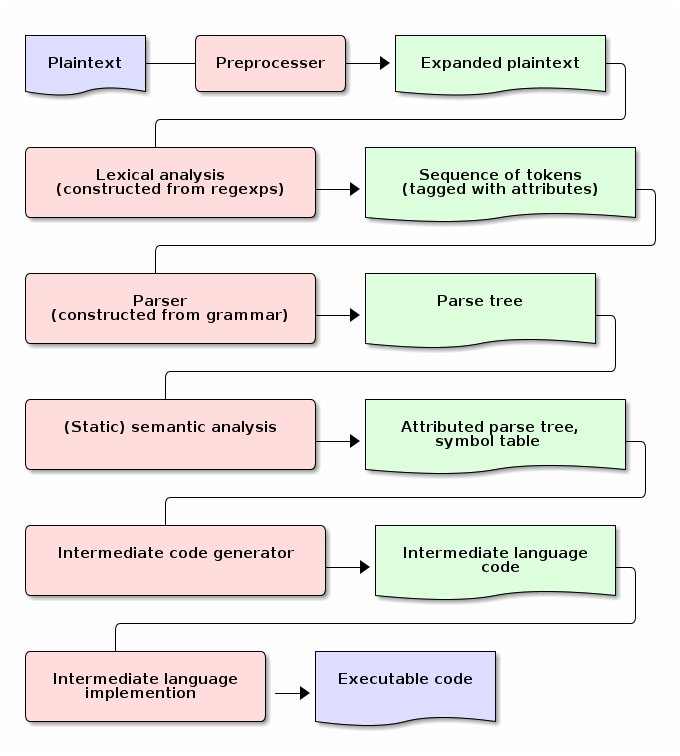
\includegraphics[width=\textwidth]{media/parsing-whole.png}
\end{center}

\section{Compilation, interpretation, and hybrid appraoches}
\label{sec:orgf4bc1ae}
We have mentioned above during the discussion of parsing
the notions of compilation and interpretation.

Let us define those terms.

\subsection{Compilation}
\label{sec:orgf94dfeb}
A \emph{compiler} translates the whole program
(and any libraries or other code resources needed)
ahead of running it.
\begin{itemize}
\item High upfront cost (time), for increased efficiency at runtime
\item Not portable; machine code is machine dependent.
\end{itemize}

\subsection{Interpreters}
\label{sec:orga4e2231}
An \emph{interpreter} translates the program \emph{as we are running it}.
\begin{itemize}
\item No upfront cost, but less efficient.
\item Portable; can be run on any machine with an interpreter.
\begin{itemize}
\item Alleviates some of the programmer's responsibility.
\begin{itemize}
\item One user (or group) writes the interpreter \emph{once}
(per machine type);
it can be used by any number of users for any number programs.
\end{itemize}
\end{itemize}
\item Efficiency is improved by using \textbf{just-in-time compilation}.
\begin{itemize}
\item Store the result of interpretation so it can be used again.
\end{itemize}
\item Can achieve better error reporting.
\begin{itemize}
\item Relationship between original and translated codes is known at runtime.
\item This relationship is discarded when compiling code.
\end{itemize}
\end{itemize}

\subsection{Hybrid methods}
\label{sec:orgfb8a43b}
\emph{Hybrid methods} compile into a special intermediate language,
which is then interpreted into machine code when the program is run.
\begin{itemize}
\item This intermediate language is usually similar to assembly.
\begin{itemize}
\item But targets a virtual machine, not actual hardware!
\end{itemize}
\item Usually called \emph{bytecode}.
\item Greatly offsets efficiency cost of interpretation.
\item More portable than compiled code; just need
a bytecode interpreter for each target machine.
\end{itemize}

\section{Ambiguity}
\label{sec:org5846edf}
We have discussed parse trees as a representation
of programs used during the parsing process.

Parse trees are extremely helpful because they allow us
to discard irrelevant details about program text,
and focus on the form of programs.

However, there is one significant problem which can occur:
what if a program has \textbf{multiple} parse trees?

It is desirable to have a single parse tree for every program.
\begin{itemize}
\item We should not admit two syntactic interpretations for a program!
\end{itemize}

This can happen quite frequently, and we must discuss
methods of eliminating such \emph{ambiguity}.

\subsection{An example of ambiguity}
\label{sec:orgf5fa90c}
For instance, the string \texttt{aa} has four valid parse trees
under the grammar
\begin{minted}[breaklines=true]{text}
⟨A⟩ ∷= a ⟨A⟩ | ⟨A⟩ a | ε 
\end{minted}

Exercise: find all four valid parse trees for \texttt{aa} with the above
grammar.

\subsection{Removing ambiguity}
\label{sec:org809ed05}
Three tools for removing ambiguity are
\begin{itemize}
\item requiring parentheses,
\item introducing precedence rules, and
\item introducing associativity rules.
\end{itemize}

The first option takes the least work on the language designer's part.
\begin{itemize}
\item But users of a language usually do not appreciate
“unnecessary” mandatory parenthesisation.
\end{itemize}

\subsection{Parentheses make structure clear}
\label{sec:orgfacd5ca}

\begin{quote}
\begin{center}
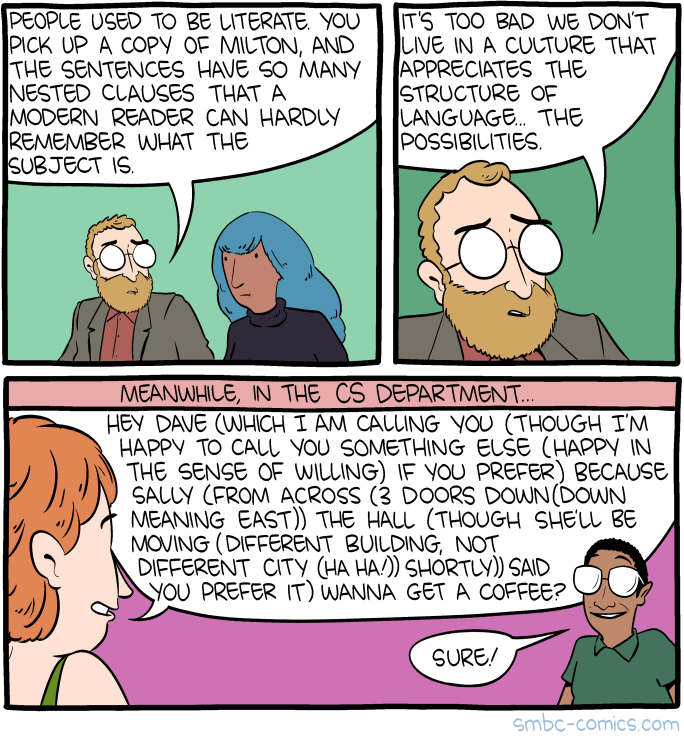
\includegraphics[width=\textwidth]{./media/comics/language.png}
\end{center}
\end{quote}
From the SMBC comic “\href{http://smbc-comics.com/comic/language}{Language}”

\subsection{Enforcing precedence with a grammar}
\label{sec:orgd04cbac}
To enforce precedence using a grammar:
\begin{itemize}
\item Create a hierarchy of non-terminals.
\item Higher-precedence operators are produced lower in the hierarchy.
\item For instance,
\begin{itemize}
\item An additive term can be an addition of multiplicative terms,
which is a multiplication of atoms, which in turn are
either a constant, variable or a \textbf{parenthesised term}.
\item Note that there is recursion in the above,
but it's “guarded” with parentheses!
\end{itemize}
\end{itemize}

For instance, if we call an additive term simply a \texttt{⟨term⟩} and
a multiplicative term a \texttt{⟨factor⟩}, we might have a grammar
\begin{minted}[breaklines=true]{text}
⟨term⟩ ∷= ⟨term⟩ + ⟨term⟩ | ⟨term⟩ - ⟨term⟩ | ⟨factor⟩
⟨factor⟩ ∷= ⟨factor⟩ * ⟨factor⟩ | ⟨factor⟩ / ⟨factor⟩
⟨atom⟩ ∷= constant | variable | '(' ⟨term⟩ ')'
\end{minted}

\subsection{Enforcing associativity with a grammar}
\label{sec:org1bf2b64}
To enforce associativity using a grammar:
\begin{itemize}
\item Left associative operators should be produced by left recursive
non-terminals.
\item And right associative operators by right recursive non-terminals.
\item Operators of the same precedence must associate the same way!
\end{itemize}

For instance, to iterate on our previous example grammar,
we might write
\begin{minted}[breaklines=true]{text}
⟨term⟩ ∷= ⟨factor⟩ + ⟨term⟩ | ⟨term⟩ - ⟨factor⟩ | ⟨factor⟩
⟨factor⟩ ∷= ⟨atom⟩ * ⟨factor⟩ | ⟨factor⟩ / ⟨atom⟩
⟨atom⟩ ∷= constant | variable | '(' ⟨term⟩ ')'
\end{minted}
Then \texttt{+} is right associative, \texttt{-} is left associative,
and similarly \texttt{*} is right associative and \texttt{/} is left associative.

\subsection{“Associative” operations}
\label{sec:org6ad7544}
You know that in mathematics,
we often avoid parentheses by declaring operations
to be \emph{left associative} or \emph{right associative}.
\begin{itemize}
\item For a left associative operator \texttt{⊕},
\texttt{a ⊕ b ⊕ c = (a ⊕ b) ⊕ c}.
\begin{itemize}
\item Examples include subtraction.
\end{itemize}
\item For a right associative operator \texttt{⊕},
\texttt{a ⊕ b ⊕ c = a ⊕ (b ⊕ c)}.
\begin{itemize}
\item Examples include exponentiation.
\end{itemize}
\item An \emph{associative} operator is a \texttt{⊕} for which
\texttt{a ⊕ b ⊕ c = (a ⊕ b) ⊕ c = a ⊕ (b ⊕ c)}.
\end{itemize}

But in computing, some operators behave differently than
their mathematical “selves”.

\subsection{Addition is not associative… in some cases}
\label{sec:orgf9a2272}

Recall that addition is an associative operator.
\begin{itemize}
\item So the choice of whether addition in a language associates to
the right or to the left may seem arbitrary.
\item But numerical types in programming are not necessarily
the same as numerical types in math!
\item Addition of floating point numbers \emph{is not associative}.
\begin{itemize}
\item Consider a binary representation with two-digit coefficients.
\item We will suffix the base with a subscript \texttt{b} to indicate
these are binary numbers.
\item \(1.0_{b} × 2^{0} + 1.0_{b} × 2^{0} + 1.0_{b} × 2^{2}\) has a different value depending
upon parenthesisation.
\end{itemize}
\end{itemize}

\begin{center}
\((1.0_{b} × 2^{0} + 1.0_{b} × 2^{0}) + 1.0_{b} × 2^{2}\ \ =\ \ 1.0_{b} × 2^{1} + 1.0_{b} × 2^{2}\ \ =\ \ 1.1_{b} × 2^{2}\)
\end{center}

\begin{center}
\(1.0_{b} × 2^{0} + (1.0_{b} × 2^{0} + 1.0_{b} × 2^{2})\ \ =\ \ 1.0_{b} × 2^{0} + 1.0_{b} × 2^{2}\ \ =\ \ 1.0_{b} × 2^{2}\)
\end{center}

\section{Abstract and concrete syntax; setting ambiguity aside}
\label{sec:org82e4bfd}
“Simple”, ambiguous grammars do have a place in describing
programming language syntax.
\begin{itemize}
\item Such grammars describe the \emph{abstract syntax} of the language.
\begin{itemize}
\item As opposed to \emph{concrete syntax}.
\end{itemize}
\item Consider programs as \emph{trees} generated by the grammar
for the abstract syntax of the language.
\begin{itemize}
\item There may be ambiguity when translating a plaintext program to a tree.
\item But once a tree representation is chosen,
\textbf{there is no ambiguity}!
\begin{itemize}
\item It may be that two different trees “flatten” to the same program,
but one tree cannot “flatten” to two different programs.
\end{itemize}
\item Such trees more efficiently represent programs.
\begin{itemize}
\item The shape of the tree expresses structure.
\item Other unnecessary details may be left out.
\end{itemize}
\end{itemize}
\end{itemize}

\subsection{Abstract syntax trees are parse trees.}
\label{sec:orgf3f4748}

We have already discussed how \emph{parse trees} are used
as an internal representation of programs
after parsing.
\begin{itemize}
\item We also stated that we discard irrelevant details during
lexical analysis and parsing (syntactic analysis.)
\begin{itemize}
\item Such as whitespace, comments, and \textbf{during parsing}, parentheses!
\end{itemize}
\end{itemize}

It is common to give two grammars for a language.
\begin{itemize}
\item The concrete grammar describes the written form of programs.
\item The abstract grammar describes the internal representation of programs.
\end{itemize}

For this reason, \emph{parse trees} are also called \emph{abstract syntax trees} (ASTs.)

\subsection{We are interested in abstract syntax}
\label{sec:orga8a2924}

For the remainder of the course, we will focus on abstract syntax.

In particular, in the discussion of the semantics of formal languages,
concrete syntactic details are not of interest to us.

\section{The \emph{semantics} of formal languages}
\label{sec:org858dcd4}
The \emph{semantics} of a language assigns a meaning to each sentence.
\begin{itemize}
\item In order to define a semantics, we must
have in mind a \emph{semantic domain};
\begin{itemize}
\item a domain of meanings into which we map sentences.
\end{itemize}
\item For instance, if we are defining a language
of natural numbers \emph{Nat}, we will map sentences into the set \texttt{ℕ}.
\item Or map elements of a languages of propositions into \texttt{𝔹}.
\item We may often provide several different definitions of
a particular mapping, to emphasise different details.
\end{itemize}

\subsection{Semantic domains}
\label{sec:org1b5b75d}

We may also have several semantic domains for a given language.
\begin{itemize}
\item In the case of programming languages,
several domains of meaning have been proposed and used;
the three most well known are
\begin{itemize}
\item computing devices, whether a real-world machine or an \emph{abstract} machine,
\begin{itemize}
\item this is known as \emph{operational semantics}
\end{itemize}
\item (mathematical) functions,
\begin{itemize}
\item this is known as \emph{denotational semantics}
\end{itemize}
\item precondition/postcondition pairs
\begin{itemize}
\item this is known as \emph{axiomatic semantics}
\end{itemize}
\end{itemize}
\end{itemize}

\subsection{Example – semantics of a language of natural numbers}
\label{sec:orgf932e15}
Consider a language of terms intended to represent
natural numbers.
\begin{minted}[breaklines=true]{text}
⟨nat⟩ ∷= zero | suc ⟨nat⟩ 
\end{minted}

To assign meaning to these terms,
we introduce a mapping from these (concrete) terms
to (abstract) numerals.
\begin{minted}[breaklines=true]{text}
eval zero = 0
eval (suc n) = (eval n) + 1
\end{minted}

The evaluation function in this case is very obvious and trivial,
because this language is simply a concrete representation
of the semantic domain.
\begin{itemize}
\item In comparison, when defining the semantics of programming languages,
the language and the semantic domain are not so directly related.
\end{itemize}

\subsection{Example – semantics of propositional logic}
\label{sec:orgd3c8abf}
As a more complex example, we can map propositional logic terms
into the set of booleans.
\begin{minted}[breaklines=true]{text}
⟨prop⟩ ∷= tt | ff | ¬ ⟨prop⟩ | ⟨prop⟩ (∧ | ∨ | ⇒ | ⇔) ⟨prop⟩
\end{minted}

In order to make the mapping less trivial, let us define it
without using boolean combinators; only constants
and “if-then-else” statements.
\begin{minted}[breaklines=true]{text}
eval tt = true
eval ff = false

eval (¬ p) = false   if eval p
             true    otherwise

eval (p ∧ q) = eval q   if eval p
               false    otherwise

…
\end{minted}
Exercise: Complete this evaluation function.

\subsection{Example – small-step semantics of propositional logic}
\label{sec:org61bdf84}
The evaluation function defined above can be considered
to be a \emph{big-step} semantics.
\begin{itemize}
\item It is a (single-valued) relation between terms and
their (final) value.
\end{itemize}

In contrast, we may define a \emph{small-step} semantics
\begin{itemize}
\item which maps terms to terms which are “one step” simpler.
\item Then, once we have reduced to a constant term, that may be mapped
to a value (this part is not shown here).
\end{itemize}
\begin{minted}[breaklines=true]{text}
reduce (¬ tt) = ff
reduce (¬ ff) = tt
reduce (¬ p)  = ¬ (reduce p)

reduce (tt ∧ q) = reduce q
reduce (ff ∧ q) = ff
reduce (p ∧ q)  = (reduce p) ∧ q

…
\end{minted}
Exercise: Complete this reduction function.
\end{document}
